% Options for packages loaded elsewhere
\PassOptionsToPackage{unicode}{hyperref}
\PassOptionsToPackage{hyphens}{url}
\PassOptionsToPackage{dvipsnames,svgnames,x11names}{xcolor}
%
\documentclass[
]{report}

\usepackage{amsmath,amssymb}
\usepackage{iftex}
\ifPDFTeX
  \usepackage[T1]{fontenc}
  \usepackage[utf8]{inputenc}
  \usepackage{textcomp} % provide euro and other symbols
\else % if luatex or xetex
  \usepackage{unicode-math}
  \defaultfontfeatures{Scale=MatchLowercase}
  \defaultfontfeatures[\rmfamily]{Ligatures=TeX,Scale=1}
\fi
\usepackage{lmodern}
\ifPDFTeX\else  
    % xetex/luatex font selection
\fi
% Use upquote if available, for straight quotes in verbatim environments
\IfFileExists{upquote.sty}{\usepackage{upquote}}{}
\IfFileExists{microtype.sty}{% use microtype if available
  \usepackage[]{microtype}
  \UseMicrotypeSet[protrusion]{basicmath} % disable protrusion for tt fonts
}{}
\makeatletter
\@ifundefined{KOMAClassName}{% if non-KOMA class
  \IfFileExists{parskip.sty}{%
    \usepackage{parskip}
  }{% else
    \setlength{\parindent}{0pt}
    \setlength{\parskip}{6pt plus 2pt minus 1pt}}
}{% if KOMA class
  \KOMAoptions{parskip=half}}
\makeatother
\usepackage{xcolor}
\setlength{\emergencystretch}{3em} % prevent overfull lines
\setcounter{secnumdepth}{-\maxdimen} % remove section numbering
% Make \paragraph and \subparagraph free-standing
\ifx\paragraph\undefined\else
  \let\oldparagraph\paragraph
  \renewcommand{\paragraph}[1]{\oldparagraph{#1}\mbox{}}
\fi
\ifx\subparagraph\undefined\else
  \let\oldsubparagraph\subparagraph
  \renewcommand{\subparagraph}[1]{\oldsubparagraph{#1}\mbox{}}
\fi

\usepackage{color}
\usepackage{fancyvrb}
\newcommand{\VerbBar}{|}
\newcommand{\VERB}{\Verb[commandchars=\\\{\}]}
\DefineVerbatimEnvironment{Highlighting}{Verbatim}{commandchars=\\\{\}}
% Add ',fontsize=\small' for more characters per line
\usepackage{framed}
\definecolor{shadecolor}{RGB}{241,243,245}
\newenvironment{Shaded}{\begin{snugshade}}{\end{snugshade}}
\newcommand{\AlertTok}[1]{\textcolor[rgb]{0.68,0.00,0.00}{#1}}
\newcommand{\AnnotationTok}[1]{\textcolor[rgb]{0.37,0.37,0.37}{#1}}
\newcommand{\AttributeTok}[1]{\textcolor[rgb]{0.40,0.45,0.13}{#1}}
\newcommand{\BaseNTok}[1]{\textcolor[rgb]{0.68,0.00,0.00}{#1}}
\newcommand{\BuiltInTok}[1]{\textcolor[rgb]{0.00,0.23,0.31}{#1}}
\newcommand{\CharTok}[1]{\textcolor[rgb]{0.13,0.47,0.30}{#1}}
\newcommand{\CommentTok}[1]{\textcolor[rgb]{0.37,0.37,0.37}{#1}}
\newcommand{\CommentVarTok}[1]{\textcolor[rgb]{0.37,0.37,0.37}{\textit{#1}}}
\newcommand{\ConstantTok}[1]{\textcolor[rgb]{0.56,0.35,0.01}{#1}}
\newcommand{\ControlFlowTok}[1]{\textcolor[rgb]{0.00,0.23,0.31}{#1}}
\newcommand{\DataTypeTok}[1]{\textcolor[rgb]{0.68,0.00,0.00}{#1}}
\newcommand{\DecValTok}[1]{\textcolor[rgb]{0.68,0.00,0.00}{#1}}
\newcommand{\DocumentationTok}[1]{\textcolor[rgb]{0.37,0.37,0.37}{\textit{#1}}}
\newcommand{\ErrorTok}[1]{\textcolor[rgb]{0.68,0.00,0.00}{#1}}
\newcommand{\ExtensionTok}[1]{\textcolor[rgb]{0.00,0.23,0.31}{#1}}
\newcommand{\FloatTok}[1]{\textcolor[rgb]{0.68,0.00,0.00}{#1}}
\newcommand{\FunctionTok}[1]{\textcolor[rgb]{0.28,0.35,0.67}{#1}}
\newcommand{\ImportTok}[1]{\textcolor[rgb]{0.00,0.46,0.62}{#1}}
\newcommand{\InformationTok}[1]{\textcolor[rgb]{0.37,0.37,0.37}{#1}}
\newcommand{\KeywordTok}[1]{\textcolor[rgb]{0.00,0.23,0.31}{#1}}
\newcommand{\NormalTok}[1]{\textcolor[rgb]{0.00,0.23,0.31}{#1}}
\newcommand{\OperatorTok}[1]{\textcolor[rgb]{0.37,0.37,0.37}{#1}}
\newcommand{\OtherTok}[1]{\textcolor[rgb]{0.00,0.23,0.31}{#1}}
\newcommand{\PreprocessorTok}[1]{\textcolor[rgb]{0.68,0.00,0.00}{#1}}
\newcommand{\RegionMarkerTok}[1]{\textcolor[rgb]{0.00,0.23,0.31}{#1}}
\newcommand{\SpecialCharTok}[1]{\textcolor[rgb]{0.37,0.37,0.37}{#1}}
\newcommand{\SpecialStringTok}[1]{\textcolor[rgb]{0.13,0.47,0.30}{#1}}
\newcommand{\StringTok}[1]{\textcolor[rgb]{0.13,0.47,0.30}{#1}}
\newcommand{\VariableTok}[1]{\textcolor[rgb]{0.07,0.07,0.07}{#1}}
\newcommand{\VerbatimStringTok}[1]{\textcolor[rgb]{0.13,0.47,0.30}{#1}}
\newcommand{\WarningTok}[1]{\textcolor[rgb]{0.37,0.37,0.37}{\textit{#1}}}

\providecommand{\tightlist}{%
  \setlength{\itemsep}{0pt}\setlength{\parskip}{0pt}}\usepackage{longtable,booktabs,array}
\usepackage{calc} % for calculating minipage widths
% Correct order of tables after \paragraph or \subparagraph
\usepackage{etoolbox}
\makeatletter
\patchcmd\longtable{\par}{\if@noskipsec\mbox{}\fi\par}{}{}
\makeatother
% Allow footnotes in longtable head/foot
\IfFileExists{footnotehyper.sty}{\usepackage{footnotehyper}}{\usepackage{footnote}}
\makesavenoteenv{longtable}
\usepackage{graphicx}
\makeatletter
\def\maxwidth{\ifdim\Gin@nat@width>\linewidth\linewidth\else\Gin@nat@width\fi}
\def\maxheight{\ifdim\Gin@nat@height>\textheight\textheight\else\Gin@nat@height\fi}
\makeatother
% Scale images if necessary, so that they will not overflow the page
% margins by default, and it is still possible to overwrite the defaults
% using explicit options in \includegraphics[width, height, ...]{}
\setkeys{Gin}{width=\maxwidth,height=\maxheight,keepaspectratio}
% Set default figure placement to htbp
\makeatletter
\def\fps@figure{htbp}
\makeatother

\makeatletter
\@ifpackageloaded{caption}{}{\usepackage{caption}}
\AtBeginDocument{%
\ifdefined\contentsname
  \renewcommand*\contentsname{Table of contents}
\else
  \newcommand\contentsname{Table of contents}
\fi
\ifdefined\listfigurename
  \renewcommand*\listfigurename{List of Figures}
\else
  \newcommand\listfigurename{List of Figures}
\fi
\ifdefined\listtablename
  \renewcommand*\listtablename{List of Tables}
\else
  \newcommand\listtablename{List of Tables}
\fi
\ifdefined\figurename
  \renewcommand*\figurename{Figure}
\else
  \newcommand\figurename{Figure}
\fi
\ifdefined\tablename
  \renewcommand*\tablename{Table}
\else
  \newcommand\tablename{Table}
\fi
}
\@ifpackageloaded{float}{}{\usepackage{float}}
\floatstyle{ruled}
\@ifundefined{c@chapter}{\newfloat{codelisting}{h}{lop}}{\newfloat{codelisting}{h}{lop}[chapter]}
\floatname{codelisting}{Listing}
\newcommand*\listoflistings{\listof{codelisting}{List of Listings}}
\makeatother
\makeatletter
\makeatother
\makeatletter
\@ifpackageloaded{caption}{}{\usepackage{caption}}
\@ifpackageloaded{subcaption}{}{\usepackage{subcaption}}
\makeatother
\ifLuaTeX
  \usepackage{selnolig}  % disable illegal ligatures
\fi
\usepackage{bookmark}

\IfFileExists{xurl.sty}{\usepackage{xurl}}{} % add URL line breaks if available
\urlstyle{same} % disable monospaced font for URLs
\hypersetup{
  colorlinks=true,
  linkcolor={blue},
  filecolor={Maroon},
  citecolor={Blue},
  urlcolor={Blue},
  pdfcreator={LaTeX via pandoc}}

\author{}
\date{2024-02-20}

\begin{document}

\chapter{Debugging PyTorch programs}\label{debugging-pytorch-programs}

\section{Getting nodes to talk to each
other}\label{getting-nodes-to-talk-to-each-other}

Once you need to use more than one node to scale your training, e.g., if
you want to use DDP to train faster, you have to get the nodes to talk
to each other, so that communication collectives could send data to each
other. This is typically done via a comms library like
\href{https://github.com/nVIDIA/nccl}{NCCL}. And in our DDP example, at
the end of training step all GPUs have to perform an
\texttt{all\_reduce} call to synchronize the gradients across all ranks.

In this section we will discuss a very simple case of just 2 nodes (with
8 GPUs each) talking to each other and which can then be easily extended
to as many nodes as needed. Let's say that these nodes have the IP
addresses 10.0.0.1 and 10.0.0.2.

Once we have the IP addresses we then need to choose a port for
communications.

In Unix there are 64k ports. The first 1k are reserved for common
services so that any computer on the Internet could connect to any other
computer knowing ahead of time which port to connect to. For example,
port 22 is reserved for SSH. So that whenever you do
\texttt{ssh\ example.com} in fact the program open a connection to
\texttt{example.com:22}.

As there are thousands of services out there, the reserved 1k ports is
not enough, and so various services could use pretty much any port. But
fear not, when you get your Linux box on the cloud or an HPC, you're
unlikely to have many preinstalled services that could use a high number
port, so most ports should be available.

Therefore let's choose port 6000.

Now we have: \texttt{10.0.0.1:6000} and \texttt{10.0.0.2:6000} that we
want to be able to communicate with each other.

The first thing to do is to open port \texttt{6000} for incoming and
outgoing connections on both nodes. It might be open already or you
might have to read up the instructions of your particular setup on how
to open a given port.

Here are multiple ways that you could use to test whether port 6000 is
already open.

\begin{Shaded}
\begin{Highlighting}[]
\ExtensionTok{telnet}\NormalTok{ localhost:6000}
\FunctionTok{nmap} \AttributeTok{{-}p}\NormalTok{ 6000 localhost}
\ExtensionTok{nc} \AttributeTok{{-}zv}\NormalTok{ localhost 6000}
\ExtensionTok{curl} \AttributeTok{{-}v}\NormalTok{ telnet://localhost:6000}
\end{Highlighting}
\end{Shaded}

Most of these should be available via \texttt{apt\ install} or whatever
your package manager uses.

Let's use \texttt{nmap} in this example. If I run:

\begin{Shaded}
\begin{Highlighting}[]
\ExtensionTok{$}\NormalTok{ nmap }\AttributeTok{{-}p}\NormalTok{ 22 localhost}
\ExtensionTok{[...]}
\ExtensionTok{PORT}\NormalTok{   STATE SERVICE}
\ExtensionTok{22/tcp}\NormalTok{ open  ssh}
\end{Highlighting}
\end{Shaded}

We can see the port is open and it tells us which protocol and service
is allocated as a bonus.

Now let's run:

\begin{Shaded}
\begin{Highlighting}[]
\ExtensionTok{$}\NormalTok{ nmap }\AttributeTok{{-}p}\NormalTok{ 6000 localhost}
\ExtensionTok{[...]}

\ExtensionTok{PORT}\NormalTok{     STATE  SERVICE}
\ExtensionTok{6000/tcp}\NormalTok{ closed X11}
\end{Highlighting}
\end{Shaded}

Here you can see port 6000 is closed.

Now that you understand how to test, you can proceed to test the
\texttt{10.0.0.1:6000} and \texttt{10.0.0.2:6000}.

First ssh to the first node in terminal A and test if port 6000 is
opened on the second node:

\begin{Shaded}
\begin{Highlighting}[]
\FunctionTok{ssh}\NormalTok{ 10.0.0.1}
\FunctionTok{nmap} \AttributeTok{{-}p}\NormalTok{ 6000 10.0.0.2}
\end{Highlighting}
\end{Shaded}

if all is good, then in terminal B ssh to the second node and do the
same check in reverse:

\begin{Shaded}
\begin{Highlighting}[]
\FunctionTok{ssh}\NormalTok{ 10.0.0.2}
\FunctionTok{nmap} \AttributeTok{{-}p}\NormalTok{ 6000 10.0.0.1}
\end{Highlighting}
\end{Shaded}

If both ports are open you can now use this port. If either or both are
closed you have to open these ports. Since most clouds use a proprietary
solution, simply search the Internet for ``open port'' and the name of
your cloud provider.

The next important thing to understand is that compute nodes will
typically have multiple network interface cards (NICs). You discover
those interfaces by running:

\begin{Shaded}
\begin{Highlighting}[]
\ExtensionTok{$}\NormalTok{ sudo ifconfig}
\end{Highlighting}
\end{Shaded}

One interface is typically used by users to connecting to nodes via ssh
or for various other non-compute related services - e.g., sending an
email or download some data. Often this interface is called
\texttt{eth0}, with \texttt{eth} standing for Ethernet, but it can be
called by other names.

Then there is the inter-node interface which can be Infiniband, EFA,
OPA, HPE Slingshot, etc. (\href{../network\#inter-node-networking}{more
information}). There could be one or dozens of those interfaces.

Here are some examples of \texttt{ifconfig}'s output:

\begin{Shaded}
\begin{Highlighting}[]
\ExtensionTok{$}\NormalTok{ sudo ifconfig}
\ExtensionTok{enp5s0:}\NormalTok{ flags=4163}\OperatorTok{\textless{}}\NormalTok{UP,BROADCAST,RUNNING,MULTICAST}\OperatorTok{\textgreater{}}\NormalTok{  mtu 1500}
        \ExtensionTok{inet}\NormalTok{ 10.0.0.23  netmask 255.255.255.0  broadcast 10.0.0.255}
        \ExtensionTok{[...]}
\end{Highlighting}
\end{Shaded}

I removed most of the output showing only some of the info. Here the key
information is the IP address that is listed after \texttt{inet}. In the
example above it's \texttt{10.0.0.23}. This is the IP address of
interface \texttt{enp5s0}.

If there is another node, it'll probably be \texttt{10.0.0.24} or
\texttt{10.0.0.21} or something of sorts - the last segment will be the
one with a different number.

Let's look at another example:

\begin{Shaded}
\begin{Highlighting}[]
\ExtensionTok{$}\NormalTok{ sudo ifconfig}
\ExtensionTok{ib0}\NormalTok{     Link encap:UNSPEC  HWaddr 00{-}00{-}00{-}00{-}00{-}00{-}00{-}00{-}00{-}00{-}00{-}00{-}00{-}00{-}00{-}00}
        \ExtensionTok{inet}\NormalTok{ addr:172.0.0.50  Bcast: 172.0.0.255  Mask:255.255.255.0}
        \ExtensionTok{[...]}
\end{Highlighting}
\end{Shaded}

Here \texttt{ib} typically tells us it's an InfiniBand card, but really
it can be any other vendor. I have seen
\href{../network\#omnipath}{OmniPath} using \texttt{ib} for example.
Again \texttt{inet} tells us the IP of this interface is
\texttt{172.0.0.50}.

If you lost me, we want the IP addresses so that we could test if
ip:port is open on each node in question.

Finally, going back to our pair of \texttt{10.0.0.1:6000} and
\texttt{10.0.0.2:6000} let's do an \texttt{all\_reduce} test using 2
terminals, where we choose \texttt{10.0.0.1} as the master host which
will coordinate other nodes. For testing we will use this helper debug
program
\href{./torch-distributed-gpu-test.py}{torch-distributed-gpu-test.py}.

In terminal A:

\begin{Shaded}
\begin{Highlighting}[]
\ExtensionTok{$}\NormalTok{ ssh 10.0.0.1}
\ExtensionTok{$}\NormalTok{ python }\AttributeTok{{-}m}\NormalTok{ torch.distributed.run }\AttributeTok{{-}{-}role} \VariableTok{$(}\FunctionTok{hostname} \AttributeTok{{-}s}\VariableTok{)}\NormalTok{: }\AttributeTok{{-}{-}tee}\NormalTok{ 3 }\AttributeTok{{-}{-}nnodes}\NormalTok{ 2 }\AttributeTok{{-}{-}nproc\_per\_node}\NormalTok{ 8 }\DataTypeTok{\textbackslash{}}
 \AttributeTok{{-}{-}master\_addr}\NormalTok{ 10.0.0.1 }\AttributeTok{{-}{-}master\_port}\NormalTok{ 6000 torch{-}distributed{-}gpu{-}test.py}
\end{Highlighting}
\end{Shaded}

In terminal B:

\begin{Shaded}
\begin{Highlighting}[]
\ExtensionTok{$}\NormalTok{ ssh 10.0.0.2}
\ExtensionTok{$}\NormalTok{ python }\AttributeTok{{-}m}\NormalTok{ torch.distributed.run }\AttributeTok{{-}{-}role} \VariableTok{$(}\FunctionTok{hostname} \AttributeTok{{-}s}\VariableTok{)}\NormalTok{: }\AttributeTok{{-}{-}tee}\NormalTok{ 3 }\AttributeTok{{-}{-}nnodes}\NormalTok{ 2 }\AttributeTok{{-}{-}nproc\_per\_node}\NormalTok{ 8 }\DataTypeTok{\textbackslash{}}
 \AttributeTok{{-}{-}master\_addr}\NormalTok{ 10.0.0.1 }\AttributeTok{{-}{-}master\_port}\NormalTok{ 6000 torch{-}distributed{-}gpu{-}test.py}
\end{Highlighting}
\end{Shaded}

Note that I'm using the same
\texttt{-\/-master\_addr\ 10.0.0.1\ -\/-master\_port\ 6000} in both
cases because we checked port 6000 is open and we use \texttt{10.0.0.1}
as the coordinating host.

This approach of running things manually from each node is painful and
so there are tools that automatically launch the same command on
multiple nodes

\textbf{pdsh}

\texttt{pdsh} is one such solution - which is like \texttt{ssh} but will
automatically run the same command on multiple nodes:

\begin{Shaded}
\begin{Highlighting}[]
\VariableTok{PDSH\_RCMD\_TYPE}\OperatorTok{=}\NormalTok{ssh }\ExtensionTok{pdsh} \AttributeTok{{-}w}\NormalTok{ 10.0.0.1,10.0.0.2 }\DataTypeTok{\textbackslash{}}
\StringTok{"python {-}m torch.distributed.run {-}{-}role }\VariableTok{$(}\FunctionTok{hostname} \AttributeTok{{-}s}\VariableTok{)}\StringTok{: {-}{-}tee 3 {-}{-}nnodes 2 {-}{-}nproc\_per\_node 8 }\DataTypeTok{\textbackslash{}}
\StringTok{ {-}{-}master\_addr 10.0.0.1 {-}{-}master\_port 6000 torch{-}distributed{-}gpu{-}test.py"}
\end{Highlighting}
\end{Shaded}

You can see how I folded the 2 sets of commands into 1. If you have more
nodes, just add more nodes as \texttt{-w} argument.

\textbf{SLURM}

If you use SLURM, it's almost certain that whoever set things up already
have all the ports opened for you, so it should just work. But if it
doesn't the information in this section should help debug things.

Here is how you'd use this with SLURM.

\begin{Shaded}
\begin{Highlighting}[]
\CommentTok{\#!/bin/bash}
\CommentTok{\#SBATCH {-}{-}job{-}name=test{-}nodes        \# name}
\CommentTok{\#SBATCH {-}{-}nodes=2                    \# nodes}
\CommentTok{\#SBATCH {-}{-}ntasks{-}per{-}node=1          \# crucial {-} only 1 task per dist per node!}
\CommentTok{\#SBATCH {-}{-}cpus{-}per{-}task=10           \# number of cores per tasks}
\CommentTok{\#SBATCH {-}{-}gres=gpu:8                 \# number of gpus}
\CommentTok{\#SBATCH {-}{-}time 0:05:00               \# maximum execution time (HH:MM:SS)}
\CommentTok{\#SBATCH {-}{-}output=\%x{-}\%j.out           \# output file name}
\CommentTok{\#}
\BuiltInTok{export} \VariableTok{GPUS\_PER\_NODE}\OperatorTok{=}\NormalTok{8}
\BuiltInTok{export} \VariableTok{MASTER\_ADDR}\OperatorTok{=}\VariableTok{$(}\ExtensionTok{scontrol}\NormalTok{ show hostnames }\VariableTok{$SLURM\_JOB\_NODELIST} \KeywordTok{|} \FunctionTok{head} \AttributeTok{{-}n}\NormalTok{ 1}\VariableTok{)}
\BuiltInTok{export} \VariableTok{MASTER\_PORT}\OperatorTok{=}\NormalTok{6000}
\CommentTok{\#}
\ExtensionTok{srun} \AttributeTok{{-}{-}jobid} \VariableTok{$SLURM\_JOBID}\NormalTok{ bash }\AttributeTok{{-}c} \StringTok{\textquotesingle{}python {-}m torch.distributed.run \textbackslash{}}
\StringTok{{-}{-}nproc\_per\_node $GPUS\_PER\_NODE {-}{-}nnodes $SLURM\_NNODES {-}{-}node\_rank $SLURM\_PROCID \textbackslash{}}
\StringTok{{-}{-}master\_addr $MASTER\_ADDR {-}{-}master\_port $MASTER\_PORT \textbackslash{}}
\StringTok{torch{-}distributed{-}gpu{-}test.py\textquotesingle{}}
\end{Highlighting}
\end{Shaded}

If you have more than 2 nodes you just need to change the number of
nodes and the above script will automatically work for any number of
them.

\textbf{MPI}:

Another popular way is to use
\href{https://en.wikipedia.org/wiki/Message_Passing_Interface}{Message
Passing Interface (MPI)}. There are a few open source implementations of
it available.

To use this tool you first create a \texttt{hostfile} that contains your
target nodes and the number of processes that should be run on each
host. In the example of this section, with 2 nodes and 8 gpus each it'd
be:

\begin{Shaded}
\begin{Highlighting}[]
\ExtensionTok{$}\NormalTok{ cat hostfile}
\ExtensionTok{10.0.0.1:8}
\ExtensionTok{10.0.0.2:8}
\end{Highlighting}
\end{Shaded}

and to run, it's just:

\begin{Shaded}
\begin{Highlighting}[]
\ExtensionTok{$}\NormalTok{ mpirun }\AttributeTok{{-}{-}hostfile}  \AttributeTok{{-}np}\NormalTok{ 16 }\AttributeTok{{-}map{-}by}\NormalTok{ ppr:8:node python my{-}program.py}
\end{Highlighting}
\end{Shaded}

Note that I used \texttt{my-program.py} here because
\href{./torch-distributed-gpu-test.py}{torch-distributed-gpu-test.py}
was written to work with \texttt{torch.distributed.run} (also known as
\texttt{torchrun}). With \texttt{mpirun} you will have to check your
specific implementation to see which environment variable it uses to
pass the rank of the program and replace \texttt{LOCAL\_RANK} with it,
the rest should be mostly the same.

Nuances: - You might have to explicitly tell it which interface to use
by adding \texttt{-\/-mca\ btl\_tcp\_if\_include\ 10.0.0.0/24} to match
our example. If you have many network interfaces it might use one that
isn't open or just the wrong interface. - You can also do the reverse
and exclude some interfaces. e.g.~say you have \texttt{docker0} and
\texttt{lo} interfaces - to exclude those add
\texttt{-\/-mca\ btl\_tcp\_if\_exclude\ docker0,lo}.

\texttt{mpirun} has a gazillion of flags and I will recommend reading
its manpage for more information. My intention was only to show you how
you could use it. Also different \texttt{mpirun} implementations may use
different CLI options.

\subsection{Solving the Infiniband connection between multiple
nodes}\label{solving-the-infiniband-connection-between-multiple-nodes}

In one situation on Azure I got 2 nodes on a shared subnet and when I
tried to run the 2 node NCCL test:

\begin{Shaded}
\begin{Highlighting}[]
\VariableTok{NCCL\_DEBUG}\OperatorTok{=}\NormalTok{INFO }\ExtensionTok{python} \AttributeTok{{-}u} \AttributeTok{{-}m}\NormalTok{ torch.distributed.run }\AttributeTok{{-}{-}nproc\_per\_node}\OperatorTok{=}\NormalTok{1 }\AttributeTok{{-}{-}nnodes}\NormalTok{ 2 }\AttributeTok{{-}{-}rdzv\_endpoint}\NormalTok{ 10.2.0.4:6000  }\AttributeTok{{-}{-}rdzv\_backend}\NormalTok{ c10d torch{-}distributed{-}gpu{-}test.py}
\end{Highlighting}
\end{Shaded}

I saw in the debug messages that Infiniband interfaces got detected:

\begin{Shaded}
\begin{Highlighting}[]
\ExtensionTok{node{-}2:5776:5898} \PreprocessorTok{[}\SpecialStringTok{0}\PreprocessorTok{]}\NormalTok{ NCCL INFO NET/IB : Using }\PreprocessorTok{[}\SpecialStringTok{0}\PreprocessorTok{]}\NormalTok{ibP111p0s0:1/IB }\PreprocessorTok{[}\SpecialStringTok{1}\PreprocessorTok{]}\NormalTok{rdmaP1111p0s2:1/RoCE }\PreprocessorTok{[}\SpecialStringTok{RO}\PreprocessorTok{]}\KeywordTok{;} \ExtensionTok{OOB}\NormalTok{ eth0:10.2.0.4}\OperatorTok{\textless{}}\NormalTok{0}\OperatorTok{\textgreater{}}
\end{Highlighting}
\end{Shaded}

But the connection would then time out with the message:

\begin{Shaded}
\begin{Highlighting}[]
\ExtensionTok{node{-}2:5776:5902} \PreprocessorTok{[}\SpecialStringTok{0}\PreprocessorTok{]}\NormalTok{ transport/net\_ib.cc:1296 NCCL WARN NET/IB : Got completion from peer 10.2.0.5}\OperatorTok{\textless{}}\NormalTok{33092}\OperatorTok{\textgreater{}}\NormalTok{ with error 12, opcode 0, len}
\ExtensionTok{0,}\NormalTok{ vendor err 129 }\ErrorTok{(}\ExtensionTok{Recv}\KeywordTok{)}
\ExtensionTok{node{-}2:5776:5902} \PreprocessorTok{[}\SpecialStringTok{0}\PreprocessorTok{]}\NormalTok{ NCCL INFO transport/net.cc:1134 }\AttributeTok{{-}}\OperatorTok{\textgreater{}}\NormalTok{ 6}
\ExtensionTok{node{-}2:5776:5902} \PreprocessorTok{[}\SpecialStringTok{0}\PreprocessorTok{]}\NormalTok{ NCCL INFO proxy.cc:679 }\AttributeTok{{-}}\OperatorTok{\textgreater{}}\NormalTok{ 6}
\ExtensionTok{node{-}2:5776:5902} \PreprocessorTok{[}\SpecialStringTok{0}\PreprocessorTok{]}\NormalTok{ NCCL INFO proxy.cc:858 }\AttributeTok{{-}}\OperatorTok{\textgreater{}}\NormalTok{ 6 [Proxy Thread]}
\end{Highlighting}
\end{Shaded}

and nothing works. So here the Ethernet connectivity between 2 nodes
works but not the IB interface.

There could be a variety of reason for this failing, but of the most
likely one is when you're on the cloud and the 2 nodes weren't
provisioned so that their IB is connected. So your Ethernet inter-node
connectivity works, but it's too slow. Chances are that you need to
re-provision the nodes so that they are allocated together. For example,
on Azure this means you have to allocate nodes within a special
\href{https://learn.microsoft.com/en-us/azure/virtual-machines/availability-set-overview?source=recommendations}{availability
set}

Going back to our case study, once the nodes were deleted and recreated
within an availability set the test worked out of the box.

The individual nodes are often not meant for inter-node communication
and often the clouds have the concept of clusters, which are designed
for allocating multiple nodes as a group and are already preconfigured
to work together.

\section{\texorpdfstring{Prefixing logs with \texttt{node:rank},
interleaved
asserts}{Prefixing logs with node:rank, interleaved asserts}}\label{prefixing-logs-with-noderank-interleaved-asserts}

In this section we will use \texttt{torchrun}
(\texttt{torch.distributed.run}) during the demonstration and at the end
of this section similar solutions for other launchers will be listed.

When you have warnings and tracebacks (or debug prints), it helps a lot
to prefix each log line with its \texttt{hostname:rank} prefix, which is
done by adding \texttt{-\/-role\ \$(hostname\ -s):\ -\/-tee\ 3} to
\texttt{torchrun}:

\begin{Shaded}
\begin{Highlighting}[]
\ExtensionTok{python} \AttributeTok{{-}m}\NormalTok{ torch.distributed.run }\AttributeTok{{-}{-}role} \VariableTok{$(}\FunctionTok{hostname} \AttributeTok{{-}s}\VariableTok{)}\NormalTok{: }\AttributeTok{{-}{-}tee}\NormalTok{ 3 }\AttributeTok{{-}{-}nnodes}\NormalTok{ 1 }\AttributeTok{{-}{-}nproc\_per\_node}\NormalTok{ 2 }\DataTypeTok{\textbackslash{}}
\NormalTok{torch{-}distributed{-}gpu{-}test.py}
\end{Highlighting}
\end{Shaded}

Now each log line will be prefixed with \texttt{{[}hostname:rank{]}}

Note that the colon is important.

If you're in a SLURM environment the above command line becomes:

\begin{Shaded}
\begin{Highlighting}[]
\ExtensionTok{srun} \AttributeTok{{-}{-}jobid} \VariableTok{$SLURM\_JOBID}\NormalTok{ bash }\AttributeTok{{-}c} \StringTok{\textquotesingle{}python {-}m torch.distributed.run \textbackslash{}}
\StringTok{{-}{-}nproc\_per\_node $GPUS\_PER\_NODE {-}{-}nnodes $SLURM\_NNODES {-}{-}node\_rank $SLURM\_PROCID \textbackslash{}}
\StringTok{{-}{-}master\_addr $MASTER\_ADDR {-}{-}master\_port $MASTER\_PORT \textbackslash{}}
\StringTok{{-}{-}role $(hostname {-}s): {-}{-}tee 3 \textbackslash{}}
\StringTok{torch{-}distributed{-}gpu{-}test.py\textquotesingle{}}
\end{Highlighting}
\end{Shaded}

Of course adjust your environment variables to match, this was just an
example.

Important! Note, that I'm using a single quoted string of commands
passed to \texttt{bash\ -c}. This way \texttt{hostname\ -s} command is
delayed until it's run on each of the nodes. If you'd use double quotes
above, \texttt{hostname\ -s} will get executed on the starting node and
then all nodes will get the same hostname as the prefix, which defeats
the purpose of using these flags. So if you use double quotes you need
to rewrite the above like so:

\begin{Shaded}
\begin{Highlighting}[]
\ExtensionTok{srun} \AttributeTok{{-}{-}jobid} \VariableTok{$SLURM\_JOBID}\NormalTok{ bash }\AttributeTok{{-}c} \StringTok{"python {-}m torch.distributed.run }\DataTypeTok{\textbackslash{}}
\StringTok{{-}{-}nproc\_per\_node }\VariableTok{$GPUS\_PER\_NODE}\StringTok{ {-}{-}nnodes }\VariableTok{$SLURM\_NNODES}\StringTok{ {-}{-}node\_rank }\DataTypeTok{\textbackslash{}$}\StringTok{SLURM\_PROCID }\DataTypeTok{\textbackslash{}}
\StringTok{{-}{-}master\_addr }\VariableTok{$MASTER\_ADDR}\StringTok{ {-}{-}master\_port }\VariableTok{$MASTER\_PORT}\StringTok{ }\DataTypeTok{\textbackslash{}}
\StringTok{{-}{-}role }\DataTypeTok{\textbackslash{}$}\StringTok{(hostname {-}s): {-}{-}tee 3 }\DataTypeTok{\textbackslash{}}
\StringTok{torch{-}distributed{-}gpu{-}test.py"}
\end{Highlighting}
\end{Shaded}

\texttt{\$SLURM\_PROCID} is escaped too as it needs to be specific to
each node and it's unknown during the launch of the slurm job on the
main node. So there are 2 \texttt{\textbackslash{}\$} escapes in this
version of the command.

This prefixing functionality is also super-helpful when one gets the
distributed program fail and which often results in interleaved
tracebacks that are very difficult to interpret. So by \texttt{grep}ing
for one \texttt{node:rank} string of choice, it's now possible to
reconstruct the real error message.

For example, if you get a traceback that looks like:

\begin{Shaded}
\begin{Highlighting}[]
  \ExtensionTok{File} \StringTok{"/path/to/training/dataset.py"}\NormalTok{, line 785, in \_\_init\_\_}
  \ExtensionTok{File} \StringTok{"/path/to/training/dataset.py"}\NormalTok{, line 785, in \_\_init\_\_}
    \ControlFlowTok{if} \FunctionTok{self.dataset\_proba.sum()} \ExtensionTok{!=}\NormalTok{ 1:}
\ExtensionTok{AttributeError:} \StringTok{\textquotesingle{}list\textquotesingle{}}\NormalTok{ object has no attribute }\StringTok{\textquotesingle{}sum\textquotesingle{}}
    \ControlFlowTok{if} \FunctionTok{self.dataset\_proba.sum()} \ExtensionTok{!=}\NormalTok{ 1:}
  \ExtensionTok{File} \StringTok{"/path/to/training/dataset.py"}\NormalTok{, line 785, in \_\_init\_\_}
  \ExtensionTok{File} \StringTok{"/path/to/training/dataset.py"}\NormalTok{, line 785, in \_\_init\_\_}
    \ControlFlowTok{if} \FunctionTok{self.dataset\_proba.sum()} \ExtensionTok{!=}\NormalTok{ 1:}
    \ControlFlowTok{if} \FunctionTok{self.dataset\_proba.sum()} \ExtensionTok{!=}\NormalTok{ 1:}
\ExtensionTok{AttributeError:} \StringTok{\textquotesingle{}list\textquotesingle{}}\NormalTok{ object has no attribute }\StringTok{\textquotesingle{}sum\textquotesingle{}}
\ExtensionTok{AttributeError:} \StringTok{\textquotesingle{}list\textquotesingle{}}\NormalTok{ object has no attribute }\StringTok{\textquotesingle{}sum\textquotesingle{}}
\ExtensionTok{AttributeError:} \StringTok{\textquotesingle{}list\textquotesingle{}}\NormalTok{ object has no attribute }\StringTok{\textquotesingle{}sum\textquotesingle{}}
\end{Highlighting}
\end{Shaded}

and when it's dozens of frames over 8 nodes it can't be made sense of,
but the above \texttt{-tee} + \texttt{-\/-role} addition will generate:

\begin{Shaded}
\begin{Highlighting}[]
\ExtensionTok{[host1:0]}\NormalTok{  File }\StringTok{"/path/to/training/dataset.py"}\NormalTok{, line 785, in \_\_init\_\_}
\ExtensionTok{[host1:1]}\NormalTok{  File }\StringTok{"/path/to/training/dataset.py"}\NormalTok{, line 785, in \_\_init\_\_}
\ExtensionTok{[host1:0]}\NormalTok{    if self.dataset\_proba.sum}\ErrorTok{(}\KeywordTok{)} \ExtensionTok{!=}\NormalTok{ 1:}
\ExtensionTok{[host1:0]AttributeError:} \StringTok{\textquotesingle{}list\textquotesingle{}}\NormalTok{ object has no attribute }\StringTok{\textquotesingle{}sum\textquotesingle{}}
\ExtensionTok{[host1:1]}\NormalTok{    if self.dataset\_proba.sum}\ErrorTok{(}\KeywordTok{)} \ExtensionTok{!=}\NormalTok{ 1:}
\ExtensionTok{[host1:2]}\NormalTok{  File }\StringTok{"/path/to/training/dataset.py"}\NormalTok{, line 785, in \_\_init\_\_}
\ExtensionTok{[host1:3]}\NormalTok{  File }\StringTok{"/path/to/training/dataset.py"}\NormalTok{, line 785, in \_\_init\_\_}
\ExtensionTok{[host1:3]}\NormalTok{    if self.dataset\_proba.sum}\ErrorTok{(}\KeywordTok{)} \ExtensionTok{!=}\NormalTok{ 1:}
\ExtensionTok{[host1:2]}\NormalTok{    if self.dataset\_proba.sum}\ErrorTok{(}\KeywordTok{)} \ExtensionTok{!=}\NormalTok{ 1:}
\ExtensionTok{[host1:1]AttributeError:} \StringTok{\textquotesingle{}list\textquotesingle{}}\NormalTok{ object has no attribute }\StringTok{\textquotesingle{}sum\textquotesingle{}}
\ExtensionTok{[host1:2]AttributeError:} \StringTok{\textquotesingle{}list\textquotesingle{}}\NormalTok{ object has no attribute }\StringTok{\textquotesingle{}sum\textquotesingle{}}
\ExtensionTok{[host1:3]AttributeError:} \StringTok{\textquotesingle{}list\textquotesingle{}}\NormalTok{ object has no attribute }\StringTok{\textquotesingle{}sum\textquotesingle{}}
\end{Highlighting}
\end{Shaded}

and you can \texttt{grep} this output for just one \texttt{host:rank}
prefix, which gives us:

\begin{Shaded}
\begin{Highlighting}[]
\ExtensionTok{$}\NormalTok{ grep }\StringTok{"[host1:0]"}\NormalTok{ log.txt}
\ExtensionTok{[host1:0]}\NormalTok{  File }\StringTok{"/path/to/training/dataset.py"}\NormalTok{, line 785, in \_\_init\_\_}
\ExtensionTok{[host1:0]}\NormalTok{    if self.dataset\_proba.sum}\ErrorTok{(}\KeywordTok{)} \ExtensionTok{!=}\NormalTok{ 1:}
\ExtensionTok{[host1:0]AttributeError:} \StringTok{\textquotesingle{}list\textquotesingle{}}\NormalTok{ object has no attribute }\StringTok{\textquotesingle{}sum\textquotesingle{}}
\end{Highlighting}
\end{Shaded}

and voila, you can now tell what really happened. And as I mentioned
earlier there can be easily a hundred to thousands of interleaved
traceback lines there.

Also, if you have just one node, you can just pass \texttt{-tee\ 3} and
there is no need to pass \texttt{-\/-role}.

If \texttt{hostname\ -s} is too long, but you have each host with its
own sequence number like:

\begin{Shaded}
\begin{Highlighting}[]
\ExtensionTok{[really{-}really{-}really{-}long{-}hostname{-}5:0]}
\ExtensionTok{[really{-}really{-}really{-}long{-}hostname{-}5:1]}
\ExtensionTok{[really{-}really{-}really{-}long{-}hostname{-}5:2]}
\end{Highlighting}
\end{Shaded}

you can of course make it shorter by replacing \texttt{hostname\ -s}
with
\texttt{hostname\ -s\ \textbar{}\ tr\ -dc\ \textquotesingle{}0-9\textquotesingle{}},
which would lead to much shorter prefixes:

\begin{Shaded}
\begin{Highlighting}[]
\ExtensionTok{[5:0]}
\ExtensionTok{[5:1]}
\ExtensionTok{[5:2]}
\end{Highlighting}
\end{Shaded}

And, of course, if you're doing debug prints, then to solve this exact
issue you can use
\href{./torch-distributed-hanging-solutions.md\#good-old-print}{\texttt{printflock}}.

Here is how you accomplish the same feat with other launchers:

\begin{itemize}
\tightlist
\item
  \texttt{srun} in SLURM: add \texttt{-\/-label}
\item
  \texttt{openmpi}: add \texttt{-\/-tag-output}
\item
  \texttt{accelerate}: you can just pass the same \texttt{-tee} +
  \texttt{-\/-role} flags as in \texttt{torchrun}
\end{itemize}

\section{Dealing with Async CUDA
bugs}\label{dealing-with-async-cuda-bugs}

When using CUDA, failing pytorch programs very often produce a python
traceback that makes no sense or can't be acted upon. This is because
due to CUDA's async nature - when a CUDA kernel is executed, the program
has already moved on and when the error happened the context of the
program isn't there. The async functionality is there to make things
faster, so that while the GPU is churning some \texttt{matmul} the
program on CPU could already start doing something else.

At other times some parts of the system will actually tell you that they
couldn't generate the correct traceback, as in this error:

\begin{Shaded}
\begin{Highlighting}[]
\ExtensionTok{[E}\NormalTok{ ProcessGroupNCCL.cpp:414] Some NCCL operations have failed or timed out. Due to the}
\ExtensionTok{asynchronous}\NormalTok{ nature of CUDA kernels, subsequent GPU operations might run on corrupted/}
\ExtensionTok{incomplete}\NormalTok{ data. To avoid this inconsistency, we are taking the entire process down.}
\end{Highlighting}
\end{Shaded}

There are a few solutions.

If the failure is instant and can be reproduced on CPU (not all programs
work on CPU), simply re-rerun it after hiding your GPUs. This is how you
do it:

\begin{Shaded}
\begin{Highlighting}[]
\VariableTok{CUDA\_VISIBLE\_DEVICES}\OperatorTok{=}\StringTok{""} \ExtensionTok{python}\NormalTok{ my{-}pytorch{-}program.py}
\end{Highlighting}
\end{Shaded}

The env var \texttt{CUDA\_VISIBLE\_DEVICES} is used to manually limit
the visibility of GPUs to the executed program. So for example if you
have 8 gpus and you want to run program1.py with first 4 gpus and
program2.py with the remaining 2 gpus you can do:

\begin{Shaded}
\begin{Highlighting}[]
\VariableTok{CUDA\_VISIBLE\_DEVICES}\OperatorTok{=}\StringTok{"0,1,2,3"} \ExtensionTok{python}\NormalTok{ my{-}pytorch{-}program1.py}
\VariableTok{CUDA\_VISIBLE\_DEVICES}\OperatorTok{=}\StringTok{"4,5,6,7"} \ExtensionTok{python}\NormalTok{ my{-}pytorch{-}program2.py}
\end{Highlighting}
\end{Shaded}

and the second program won't be the wiser that it's not using GPUs 0-3.

But in the case of debug we are hiding all GPUs, by setting
\texttt{CUDA\_VISIBLE\_DEVICES=""}.

Now the program runs on CPU and you will get a really nice traceback and
will fix the problem in no time.

But, of course, if you your program requires multiple GPUs this won't
work. And so here is another solution.

Rerun your program after setting this environment variable:

\begin{Shaded}
\begin{Highlighting}[]
\VariableTok{CUDA\_LAUNCH\_BLOCKING}\OperatorTok{=}\NormalTok{1 }\ExtensionTok{python}\NormalTok{ my{-}pytorch{-}program.py}
\end{Highlighting}
\end{Shaded}

This variable tells pytorch (or any other CUDA-based program) to turn
its async nature off everywhere and now all operations will be
synchronous. So when the program crashes you should now get a perfect
traceback and you will know exactly what ails your program.

In theory enabling this variable should make everything run really slow,
but in reality it really depends on your software. We did the whole of
BLOOM-176B training using \texttt{CUDA\_LAUNCH\_BLOCKING=1} with
\texttt{Megatron-Deepspeed}{]}(https://github.com/bigscience-workshop/Megatron-DeepSpeed)
and had zero slowdown - we had to use it as pytorch was hanging without
it and we had no time to figure the hanging out.

So, yes, when you switch from async to sync nature, often it can hide
some subtle race conditions, so there are times that a hanging
disappears as in the example I shared above. So measure your throughput
with and without this flag and sometimes it might actual not only help
with getting an in-context traceback but actually solve your problem
altogether.

Note: \href{https://github.com/NVIDIA/nccl/issues/750}{NCCL==2.14.3
coming with \texttt{pytorch==1.13} hangs} when
\texttt{CUDA\_LAUNCH\_BLOCKING=1} is used. So don't use it with that
version of pytorch. The issue has been fixed in
\texttt{nccl\textgreater{}=2.17} which should be included in
\texttt{pytorch==2.0}.

\section{segfaults and getting a backtrace from a core
file}\label{segfaults-and-getting-a-backtrace-from-a-core-file}

It's not uncommon for a complex pytorch program to segfault and drop a
core file. Especially if you're using complex extensions like NCCL.

The corefile is what the program generates when it crashes on a
low-level - e.g.~when using a python extension - such as a CUDA kernel
or really any library that is coded directly in some variant of C or
another language and made accessible in python through some binding API.
The most common cause of a segfault is when such software accesses
memory it has not allocated. For example, a program may try to free
memory it hasn't allocated. But there could be many other reasons.

When a segfault event happens Python can't do anything, as the
proverbial carpet is pulled out from under its feet, so it can't
generate an exception or even write anything to the output.

In these situation one must go and analyse the libC-level calls that
lead to the segfault, which is luckily saved in the core file.

If your program crashed, you will often find a file that will look
something like: \texttt{core-python-3097667-6}

Before we continue make sure you have \texttt{gdb} installed:

\begin{Shaded}
\begin{Highlighting}[]
\FunctionTok{sudo}\NormalTok{ apt{-}get install gdb}
\end{Highlighting}
\end{Shaded}

Now make sure you know the path to the python executable that was used
to run the program that crashed. If you have multiple python environment
you have to activate the right environment first. If you don't
\texttt{gdb} may fail to unpack the core file.

So typically I'd go:

\begin{Shaded}
\begin{Highlighting}[]
\ExtensionTok{conda}\NormalTok{ activate my{-}env}
\FunctionTok{gdb}\NormalTok{ python core{-}python{-}3097667{-}6}
\end{Highlighting}
\end{Shaded}

\begin{itemize}
\tightlist
\item
  adjust \texttt{my-env} to whatever env you use, or instead of conda
  use whatever way you use to activate your python environment - and
  perhaps you're using the system-wise python and then you don't need to
  activate anything.
\item
  adjust the name of the core file to the file you have gotten - it's
  possible that there are many - pick the latest then.
\end{itemize}

Now \texttt{gdb} will churn for a bit and will give you a prompt where
you type: \texttt{bt}. We will use an actual core file here:

\begin{Shaded}
\begin{Highlighting}[]
\KeywordTok{(}\FunctionTok{gdb}\KeywordTok{)} \ExtensionTok{bt}
\CommentTok{\#0  0x0000147539887a9f in raise () from /lib64/libc.so.6}
\CommentTok{\#1  0x000014753985ae05 in abort () from /lib64/libc.so.6}
\CommentTok{\#2  0x000014751b85a09b in \_\_gnu\_cxx::\_\_verbose\_terminate\_handler() [clone .cold.1] () from /lib64/libstdc++.so.6}
\CommentTok{\#3  0x000014751b86053c in \_\_cxxabiv1::\_\_terminate(void (*)()) () from /lib64/libstdc++.so.6}
\CommentTok{\#4  0x000014751b860597 in std::terminate() () from /lib64/libstdc++.so.6}
\CommentTok{\#5  0x000014751b86052e in std::rethrow\_exception(std::\_\_exception\_ptr::exception\_ptr) () from /lib64/libstdc++.so.6}
\CommentTok{\#6  0x000014750bb007ef in c10d::ProcessGroupNCCL::WorkNCCL::handleNCCLGuard() ()}
   \ExtensionTok{from}\NormalTok{ .../python3.8/site{-}packages/torch/lib/libtorch\_cuda\_cpp.so}
\CommentTok{\#7  0x000014750bb04c69 in c10d::ProcessGroupNCCL::workCleanupLoop() ()}
   \ExtensionTok{from.../python3.8/site{-}packages/torch/lib/libtorch\_cuda\_cpp.so}
\CommentTok{\#8  0x000014751b88cba3 in execute\_native\_thread\_routine () from /lib64/libstdc++.so.6}
\CommentTok{\#9  0x000014753a3901cf in start\_thread () from /lib64/libpthread.so.0}
\CommentTok{\#10 0x0000147539872dd3 in clone () from /lib64/libc.so.6}
\end{Highlighting}
\end{Shaded}

and there you go. How do you make sense of it?

Well, you go from the bottom of the stack to the top. You can tell that
a \texttt{clone} call was made in \texttt{libc} which then called
\texttt{start\_thread} in \texttt{libpthread} and then if you keep going
there are a bunch of calls in the torch libraries and finally we can see
that the program terminated itself, completing with \texttt{raise} from
\texttt{libc} which told the Linux kernel to kill the program and create
the core file.

This wasn't an easy to understand backtrace.

footnote: Yes, python calls it a \emph{traceback} and elsewhere it's
called a \emph{backtrace} - it's confusing, but it's more or less the
same thing.

Actually I had to ask pytorch devs for help and received:

\begin{itemize}
\tightlist
\item
  PyTorch \texttt{ProcessGroup} watchdog thread caught an asynchronous
  error from NCCL
\item
  This error is an \texttt{“unhandled\ system\ error”} which in this
  particular case turned out to be an IB-OPA error
\item
  The \texttt{ProcessGroup}'s \texttt{WorkCleanUp} thread rethrew the
  error so that the main process would crash and the user would get
  notified (otherwise this async error would not surface)
\end{itemize}

Trust me there are times when even if you're inexperienced the backtrace
can give you enough of a hint to where you should look for
troubleshooting.

But fear not - most of the time you won't need to understand the
traceback. Ideally you'd just attach the core file to your filed Issue.
But it can easily be 5GB large. So the developers that will be trying to
help you will ask you to generate a \texttt{gdb} backtrace and now you
know how to do that.

I didn't promise it'll be easy, I just showed you where to start.

Now another useful details is that many programs these days run multiple
threads. And \texttt{bt} only shows the main thread of the process. But,
often, it can be helpful to see where other threads in the process were
when segfault has happened. For that you simply type 2 commands at the
\texttt{(gdb)} prompt:

\begin{Shaded}
\begin{Highlighting}[]
\KeywordTok{(}\FunctionTok{gdb}\KeywordTok{)} \ExtensionTok{thread}\NormalTok{ apply all bt}
\KeywordTok{(}\FunctionTok{gdb}\KeywordTok{)} \ExtensionTok{bt}
\end{Highlighting}
\end{Shaded}

and this time around you typically will get a massive report, one
backtrace per thread.

\section{py-spy}\label{py-spy}

This is a super-useful tool for analysing hanging programs. For example,
when a you have a resource deadlock or there is an issue with a network
connection.

You will find an exhaustive coverage of this tool
\href{./torch-distributed-hanging-solutions.md\#py-spy}{here}.

\section{strace}\label{strace}

Similar to
\href{./torch-distributed-hanging-solutions.md\#py-spy}{py-spy},
\texttt{strace} is a super-useful tool which traces any running
application at the low-level system calls - e.g.~\texttt{libC} and
alike.

For example, run:

\begin{Shaded}
\begin{Highlighting}[]
\ExtensionTok{strace}\NormalTok{ python }\AttributeTok{{-}c} \StringTok{"print(\textquotesingle{}strace\textquotesingle{})"}
\end{Highlighting}
\end{Shaded}

and you will see everything that is done at the system call level as the
above program runs.

But usually it's more useful when you have a stuck program that spins
all CPU cores at 100\% but nothing happens and you want to see what's it
doing. In this situation you simply attached to the running program like
so:

\begin{Shaded}
\begin{Highlighting}[]
\ExtensionTok{strace} \AttributeTok{{-}{-}pid}\NormalTok{ PID}
\end{Highlighting}
\end{Shaded}

where you get the PID for example from the output of \texttt{top} or
\texttt{ps}. Typically I just copy-n-paste the PID of the program that
consumes the most CPU - \texttt{top} usually shows it at the very top of
its listing.

Same as \texttt{py-spy} you may need \texttt{sudo} perms to attached to
an already running process - it all depends on your system setup. But
you can always start a program with \texttt{strace} as I have shown in
the original example.

Let's look at a small sub-snippet of the output of
\texttt{strace\ python\ -c\ "print(\textquotesingle{}strace\textquotesingle{})"}

\begin{Shaded}
\begin{Highlighting}[]
\FunctionTok{write}\ErrorTok{(}\ExtensionTok{1,} \StringTok{"strace\textbackslash{}n"}\NormalTok{, 7strace}
\KeywordTok{)}                 \ExtensionTok{=}\NormalTok{ 7}
\end{Highlighting}
\end{Shaded}

Here we can see that a write call was executed on filedescriptor
\texttt{1}, which almost always is \texttt{stdout} (\texttt{stdin} being
0, and \texttt{stderr} being 2).

If you're not sure what a filedescriptor is pointing to, normally you
can tell from \texttt{strace}'s output itself. But you can also do:

\begin{Shaded}
\begin{Highlighting}[]
\FunctionTok{ls} \AttributeTok{{-}l}\NormalTok{ /proc/PID/fd}
\end{Highlighting}
\end{Shaded}

where PID is the pid of the currently running program you're trying to
investigate.

For example, when I run the above while running a pytest test with gpus,
I got (partial output):

\begin{Shaded}
\begin{Highlighting}[]
\ExtensionTok{l{-}wx{-}{-}{-}{-}{-}{-}}\NormalTok{ 1 stas stas 64 Mar  1 17:22 5 }\AttributeTok{{-}}\OperatorTok{\textgreater{}}\NormalTok{ /dev/null}
\ExtensionTok{lr{-}x{-}{-}{-}{-}{-}{-}}\NormalTok{ 1 stas stas 64 Mar  1 17:22 6 }\AttributeTok{{-}}\OperatorTok{\textgreater{}}\NormalTok{ /dev/urandom}
\ExtensionTok{lrwx{-}{-}{-}{-}{-}{-}}\NormalTok{ 1 stas stas 64 Mar  1 17:22 7 }\AttributeTok{{-}}\OperatorTok{\textgreater{}}\NormalTok{ /dev/nvidiactl}
\ExtensionTok{lrwx{-}{-}{-}{-}{-}{-}}\NormalTok{ 1 stas stas 64 Mar  1 17:22 8 }\AttributeTok{{-}}\OperatorTok{\textgreater{}}\NormalTok{ /dev/nvidia0}
\ExtensionTok{lr{-}x{-}{-}{-}{-}{-}{-}}\NormalTok{ 1 stas stas 64 Mar  1 17:22 9 }\AttributeTok{{-}}\OperatorTok{\textgreater{}}\NormalTok{ /dev/nvidia{-}caps/nvidia{-}cap2}
\end{Highlighting}
\end{Shaded}

so you can see that a device \texttt{/dev/null} is open as FD (file
descriptor) 5, \texttt{/dev/urandom} as FD 6, etc.

Now let's go look at another snippet from our \texttt{strace} run.

\begin{Shaded}
\begin{Highlighting}[]
\ExtensionTok{access}\ErrorTok{(}\StringTok{"/etc/ld.so.preload"}\ExtensionTok{,}\NormalTok{ R\_OK}\KeywordTok{)}      \ExtensionTok{=} \AttributeTok{{-}1}\NormalTok{ ENOENT }\ErrorTok{(}\ExtensionTok{No}\NormalTok{ such file or directory}\KeywordTok{)}
\end{Highlighting}
\end{Shaded}

Here it tried to see if file \texttt{/etc/ld.so.preload} exists, but as
we can see it doesn't - this can be useful if some shared library is
missing - you can see where it's trying to load it from.

Let's try another one:

\begin{Shaded}
\begin{Highlighting}[]
\ExtensionTok{openat}\ErrorTok{(}\ExtensionTok{AT\_FDCWD,} \StringTok{"/lib/x86\_64{-}linux{-}gnu/libpthread.so.0"}\NormalTok{, O\_RDONLY}\KeywordTok{|}\ExtensionTok{O\_CLOEXEC}\KeywordTok{)} \ExtensionTok{=}\NormalTok{ 3}
\BuiltInTok{read}\ErrorTok{(}\ExtensionTok{3,} \StringTok{"\textbackslash{}177ELF\textbackslash{}2\textbackslash{}1\textbackslash{}1\textbackslash{}0\textbackslash{}0\textbackslash{}0\textbackslash{}0\textbackslash{}0\textbackslash{}0\textbackslash{}0\textbackslash{}0\textbackslash{}0\textbackslash{}3\textbackslash{}0\textgreater{}\textbackslash{}0\textbackslash{}1\textbackslash{}0\textbackslash{}0\textbackslash{}0\textbackslash{}0\textbackslash{}0\textbackslash{}0\textbackslash{}0\textbackslash{}0\textbackslash{}0\textbackslash{}0\textbackslash{}0"}\NormalTok{..., 832}\KeywordTok{)} \ExtensionTok{=}\NormalTok{ 832}
\ExtensionTok{newfstatat}\ErrorTok{(}\ExtensionTok{3,} \StringTok{""}\NormalTok{, \{st\_mode=S\_IFREG}\KeywordTok{|}\ExtensionTok{0644,}\NormalTok{ st\_size=21448, ...\}, AT\_EMPTY\_PATH}\KeywordTok{)} \ExtensionTok{=}\NormalTok{ 0}
\ExtensionTok{mmap}\ErrorTok{(}\ExtensionTok{NULL,}\NormalTok{ 16424, PROT\_READ, MAP\_PRIVATE}\KeywordTok{|}\ExtensionTok{MAP\_DENYWRITE,}\NormalTok{ 3, 0}\KeywordTok{)} \ExtensionTok{=}\NormalTok{ 0x7f8028807000}
\ExtensionTok{mmap}\ErrorTok{(}\ExtensionTok{0x7f8028808000,}\NormalTok{ 4096, PROT\_READ}\KeywordTok{|}\ExtensionTok{PROT\_EXEC,}\NormalTok{ MAP\_PRIVATE}\KeywordTok{|}\ExtensionTok{MAP\_FIXED}\KeywordTok{|}\ExtensionTok{MAP\_DENYWRITE,}\NormalTok{ 3, 0x1000}\KeywordTok{)} \ExtensionTok{=}\NormalTok{ 0x7f8028808000}
\ExtensionTok{mmap}\ErrorTok{(}\ExtensionTok{0x7f8028809000,}\NormalTok{ 4096, PROT\_READ, MAP\_PRIVATE}\KeywordTok{|}\ExtensionTok{MAP\_FIXED}\KeywordTok{|}\ExtensionTok{MAP\_DENYWRITE,}\NormalTok{ 3, 0x2000}\KeywordTok{)} \ExtensionTok{=}\NormalTok{ 0x7f8028809000}
\ExtensionTok{mmap}\ErrorTok{(}\ExtensionTok{0x7f802880a000,}\NormalTok{ 8192, PROT\_READ}\KeywordTok{|}\ExtensionTok{PROT\_WRITE,}\NormalTok{ MAP\_PRIVATE}\KeywordTok{|}\ExtensionTok{MAP\_FIXED}\KeywordTok{|}\ExtensionTok{MAP\_DENYWRITE,}\NormalTok{ 3, 0x2000}\KeywordTok{)} \ExtensionTok{=}\NormalTok{ 0x7f802880a000}
\ExtensionTok{close}\ErrorTok{(}\ExtensionTok{3}\KeywordTok{)}
\end{Highlighting}
\end{Shaded}

here we can see that it opens
\texttt{/lib/x86\_64-linux-gnu/libpthread.so.0} and assigns it FD 3, it
then reads 832 chars from FD 3, (we can also see that the first chars
are ELF - which stands for a shared library format), then memory maps it
and closes that file.

In this following example, we see a python cached file is opened, its
filepointer is moved to 0, and then it's read and closed.

\begin{Shaded}
\begin{Highlighting}[]
\ExtensionTok{openat}\ErrorTok{(}\ExtensionTok{AT\_FDCWD,} \StringTok{"/home/stas/anaconda3/envs/py38{-}pt113/lib/python3.8/\_\_pycache\_\_/abc.cpython{-}38.pyc"}\NormalTok{, O\_RDONLY}\KeywordTok{|}\ExtensionTok{O\_CLOEXEC}\KeywordTok{)} \ExtensionTok{=}\NormalTok{ 3}
\ExtensionTok{fstat}\ErrorTok{(}\ExtensionTok{3,}\NormalTok{ \{st\_mode=S\_IFREG}\KeywordTok{|}\ExtensionTok{0664,}\NormalTok{ st\_size=5329, ...\}}\KeywordTok{)} \ExtensionTok{=}\NormalTok{ 0}
\ExtensionTok{lseek}\ErrorTok{(}\ExtensionTok{3,}\NormalTok{ 0, SEEK\_CUR}\KeywordTok{)}                   \ExtensionTok{=}\NormalTok{ 0}
\ExtensionTok{lseek}\ErrorTok{(}\ExtensionTok{3,}\NormalTok{ 0, SEEK\_CUR}\KeywordTok{)}                   \ExtensionTok{=}\NormalTok{ 0}
\ExtensionTok{fstat}\ErrorTok{(}\ExtensionTok{3,}\NormalTok{ \{st\_mode=S\_IFREG}\KeywordTok{|}\ExtensionTok{0664,}\NormalTok{ st\_size=5329, ...\}}\KeywordTok{)} \ExtensionTok{=}\NormalTok{ 0}
\ExtensionTok{brk}\ErrorTok{(}\ExtensionTok{0x23bf000}\KeywordTok{)}                          \ExtensionTok{=}\NormalTok{ 0x23bf000}
\BuiltInTok{read}\ErrorTok{(}\ExtensionTok{3,} \StringTok{"U\textbackslash{}r\textbackslash{}r\textbackslash{}n\textbackslash{}0\textbackslash{}0\textbackslash{}0\textbackslash{}0\textbackslash{}24\textbackslash{}216\textbackslash{}177c\textbackslash{}211\textbackslash{}21\textbackslash{}0\textbackslash{}0\textbackslash{}343\textbackslash{}0\textbackslash{}0\textbackslash{}0\textbackslash{}0\textbackslash{}0\textbackslash{}0\textbackslash{}0\textbackslash{}0\textbackslash{}0\textbackslash{}0\textbackslash{}0\textbackslash{}0\textbackslash{}0\textbackslash{}0\textbackslash{}0"}\NormalTok{..., 5330}\KeywordTok{)} \ExtensionTok{=}\NormalTok{ 5329}
\BuiltInTok{read}\ErrorTok{(}\ExtensionTok{3,} \StringTok{""}\NormalTok{, 1}\KeywordTok{)}                          \ExtensionTok{=}\NormalTok{ 0}
\ExtensionTok{close}\ErrorTok{(}\ExtensionTok{3}\KeywordTok{)}
\end{Highlighting}
\end{Shaded}

It's important to notice that file descriptors are re-used, so we have
seen the same FD 3 twice, but each time it was open to a different file.

If your program is for example trying to reach to the Internet, you can
also tell these calls from \texttt{strace} as the program would be
reading from a socket file descriptor.

So let's run an example on a program that downloads files from the HF
hub:

\begin{Shaded}
\begin{Highlighting}[]
\ExtensionTok{strace}\NormalTok{ python }\AttributeTok{{-}c} \StringTok{\textquotesingle{}import sys; from transformers import AutoConfig; AutoConfig.from\_pretrained(sys.argv[1])\textquotesingle{}}\NormalTok{ t5{-}small}
\end{Highlighting}
\end{Shaded}

here is some relevant to this discussion snippet:

\begin{Shaded}
\begin{Highlighting}[]
\ExtensionTok{socket}\ErrorTok{(}\ExtensionTok{AF\_INET6,}\NormalTok{ SOCK\_STREAM}\KeywordTok{|}\ExtensionTok{SOCK\_CLOEXEC,}\NormalTok{ IPPROTO\_TCP}\KeywordTok{)} \ExtensionTok{=}\NormalTok{ 3}
\ExtensionTok{setsockopt}\ErrorTok{(}\ExtensionTok{3,}\NormalTok{ SOL\_TCP, TCP\_NODELAY, }\PreprocessorTok{[}\SpecialStringTok{1}\PreprocessorTok{]}\NormalTok{, 4}\KeywordTok{)} \ExtensionTok{=}\NormalTok{ 0}
\ExtensionTok{ioctl}\ErrorTok{(}\ExtensionTok{3,}\NormalTok{ FIONBIO, }\PreprocessorTok{[}\SpecialStringTok{1}\PreprocessorTok{]}\KeywordTok{)}                  \ExtensionTok{=}\NormalTok{ 0}
\ExtensionTok{connect}\ErrorTok{(}\ExtensionTok{3,}\NormalTok{ \{sa\_family=AF\_INET6, sin6\_port=htons}\ErrorTok{(}\ExtensionTok{443}\KeywordTok{)}\ExtensionTok{,}\NormalTok{ sin6\_flowinfo=htonl}\ErrorTok{(}\ExtensionTok{0}\KeywordTok{)}\ExtensionTok{,}\NormalTok{ inet\_pton}\ErrorTok{(}\ExtensionTok{AF\_INET6,} \StringTok{"2600:1f18:147f:e850:e203:c458:10cd:fc3c}
\StringTok{"}\NormalTok{, }\KeywordTok{\&}\ExtensionTok{sin6\_addr}\KeywordTok{)}\ExtensionTok{,}\NormalTok{ sin6\_scope\_id=0\}, 28}\KeywordTok{)} \ExtensionTok{=} \AttributeTok{{-}1}\NormalTok{ EINPROGRESS }\ErrorTok{(}\ExtensionTok{Operation}\NormalTok{ now in progress}\KeywordTok{)}
\ExtensionTok{poll}\ErrorTok{(}\ExtensionTok{[\{fd=3,}\NormalTok{ events=POLLOUT}\KeywordTok{|}\ExtensionTok{POLLERR\}],}\NormalTok{ 1, 10000}\KeywordTok{)} \ExtensionTok{=}\NormalTok{ 1 }\ErrorTok{(}\ExtensionTok{[\{fd=3,}\NormalTok{ revents=POLLOUT\}]}\KeywordTok{)}
\ExtensionTok{getsockopt}\ErrorTok{(}\ExtensionTok{3,}\NormalTok{ SOL\_SOCKET, SO\_ERROR, }\PreprocessorTok{[}\SpecialStringTok{0}\PreprocessorTok{]}\NormalTok{, }\PreprocessorTok{[}\SpecialStringTok{4}\PreprocessorTok{]}\KeywordTok{)} \ExtensionTok{=}\NormalTok{ 0}
\ExtensionTok{[...]}
\FunctionTok{write}\ErrorTok{(}\ExtensionTok{3,} \StringTok{"\textbackslash{}26\textbackslash{}3\textbackslash{}3\textbackslash{}0F\textbackslash{}20\textbackslash{}0\textbackslash{}0BA\textbackslash{}4\textbackslash{}373m\textbackslash{}244\textbackslash{}16\textbackslash{}354/\textbackslash{}334\textbackslash{}205\textbackslash{}361j\textbackslash{}225\textbackslash{}356\textbackslash{}202m*\textbackslash{}305\textbackslash{}332\textbackslash{}275\textbackslash{}251\textbackslash{}17J"}\NormalTok{..., 126}\KeywordTok{)} \ExtensionTok{=}\NormalTok{ 126}
\BuiltInTok{read}\ErrorTok{(}\ExtensionTok{3,}\NormalTok{ 0x2f05c13, 5}\KeywordTok{)}                   \ExtensionTok{=} \AttributeTok{{-}1}\NormalTok{ EAGAIN }\ErrorTok{(}\ExtensionTok{Resource}\NormalTok{ temporarily unavailable}\KeywordTok{)}
\ExtensionTok{poll}\ErrorTok{(}\ExtensionTok{[\{fd=3,}\NormalTok{ events=POLLIN\}], 1, 9903}\KeywordTok{)}  \ExtensionTok{=}\NormalTok{ 1 }\ErrorTok{(}\ExtensionTok{[\{fd=3,}\NormalTok{ revents=POLLIN\}]}\KeywordTok{)}
\BuiltInTok{read}\ErrorTok{(}\ExtensionTok{3,} \StringTok{"\textbackslash{}24\textbackslash{}3\textbackslash{}3\textbackslash{}0\textbackslash{}1"}\NormalTok{, 5}\KeywordTok{)}               \ExtensionTok{=}\NormalTok{ 5}
\BuiltInTok{read}\ErrorTok{(}\ExtensionTok{3,} \StringTok{"\textbackslash{}1"}\NormalTok{, 1}\KeywordTok{)}                        \ExtensionTok{=}\NormalTok{ 1}
\BuiltInTok{read}\ErrorTok{(}\ExtensionTok{3,} \StringTok{"\textbackslash{}26\textbackslash{}3\textbackslash{}3\textbackslash{}0("}\NormalTok{, 5}\KeywordTok{)}                \ExtensionTok{=}\NormalTok{ 5}
\BuiltInTok{read}\ErrorTok{(}\ExtensionTok{3,} \StringTok{"\textbackslash{}0\textbackslash{}0\textbackslash{}0\textbackslash{}0\textbackslash{}0\textbackslash{}0\textbackslash{}0\textbackslash{}0\textbackslash{}344\textbackslash{}v\textbackslash{}273\textbackslash{}225}\KeywordTok{\textasciigrave{}}\ExtensionTok{\textbackslash{}4\textbackslash{}24m\textbackslash{}234\textasciitilde{}\textbackslash{}371\textbackslash{}332\%l\textbackslash{}364\textbackslash{}254\textbackslash{}34\textbackslash{}3472}\OperatorTok{\textless{}}\DataTypeTok{\textbackslash{}0}\NormalTok{356s\textbackslash{}313}\StringTok{"..., 40) = 40}
\StringTok{ioctl(3, FIONBIO, [1])                  = 0}
\StringTok{poll([\{fd=3, events=POLLOUT\}], 1, 10000) = 1 ([\{fd=3, revents=POLLOUT\}])}
\StringTok{write(3, "}\DataTypeTok{\textbackslash{}2}\NormalTok{7\textbackslash{}3\textbackslash{}3\textbackslash{}1.\textbackslash{}0\textbackslash{}374$}\DataTypeTok{\textbackslash{}3}\NormalTok{61\textbackslash{}217\textbackslash{}337\textbackslash{}377\textbackslash{}264g\textbackslash{}215\textbackslash{}364\textbackslash{}345\textbackslash{}256\textbackslash{}260\textbackslash{}211$}\DataTypeTok{\textbackslash{}3}\NormalTok{26pkR\textbackslash{}345\textbackslash{}276,\textbackslash{}321\textbackslash{}221}\KeywordTok{\textasciigrave{}}\StringTok{{-}"}\NormalTok{..., 307}\KeywordTok{)} \ExtensionTok{=}\NormalTok{ 307}
\ExtensionTok{ioctl}\ErrorTok{(}\ExtensionTok{3,}\NormalTok{ FIONBIO, }\PreprocessorTok{[}\SpecialStringTok{1}\PreprocessorTok{]}\KeywordTok{)}                  \ExtensionTok{=}\NormalTok{ 0}
\BuiltInTok{read}\ErrorTok{(}\ExtensionTok{3,}\NormalTok{ 0x2ef7283, 5}\KeywordTok{)}                   \ExtensionTok{=} \AttributeTok{{-}1}\NormalTok{ EAGAIN }\ErrorTok{(}\ExtensionTok{Resource}\NormalTok{ temporarily unavailable}\KeywordTok{)}
\ExtensionTok{poll}\ErrorTok{(}\ExtensionTok{[\{fd=3,}\NormalTok{ events=POLLIN\}], 1, 10000}\KeywordTok{)} \ExtensionTok{=}\NormalTok{ 1 }\ErrorTok{(}\ExtensionTok{[\{fd=3,}\NormalTok{ revents=POLLIN\}]}\KeywordTok{)}
\end{Highlighting}
\end{Shaded}

You can see where that again it uses FD 3 but this time it opens a INET6
socket instead of a file. You can see that it then connects to that
socket, polls, reads and writes from it.

There are many other super useful understandings one can derive from
using this tool.

BTW, if you don't want to scroll up-down, you can also save the output
to a file:

\begin{Shaded}
\begin{Highlighting}[]
\ExtensionTok{strace} \AttributeTok{{-}o}\NormalTok{ strace.txt python }\AttributeTok{{-}c} \StringTok{"print(\textquotesingle{}strace\textquotesingle{})"}
\end{Highlighting}
\end{Shaded}

Now, since you're might want to strace the program from the very
beginning, for example to sort out some race condition on a distributed
filesystem, you will want to tell it to follow any forked processes.
This what the \texttt{-f} flag is for:

\begin{Shaded}
\begin{Highlighting}[]
\ExtensionTok{strace} \AttributeTok{{-}o}\NormalTok{ log.txt }\AttributeTok{{-}f}\NormalTok{ python }\AttributeTok{{-}m}\NormalTok{ torch.distributed.run }\AttributeTok{{-}{-}nproc\_per\_node}\OperatorTok{=}\NormalTok{4 }\AttributeTok{{-}{-}nnodes}\OperatorTok{=}\NormalTok{1 }\AttributeTok{{-}{-}tee}\NormalTok{ 3 test.py}
\end{Highlighting}
\end{Shaded}

So here we launch 4 processes and will end up running \texttt{strace} on
at least 5 of them - the launcher plus 4 processes (each of which may
spawn further child processes).

It will conveniently prefix each line with the pid of the program so it
should be easy to tell which system was made by which process.

But if you want separate logs per process, then use \texttt{-ff} instead
of \texttt{-f}.

The \texttt{strace} manpage has a ton of other useful options.

\section{Invoke pdb on a specific rank in multi-node
training}\label{invoke-pdb-on-a-specific-rank-in-multi-node-training}

Once pytorch 2.2 is released you will have a new handy debug feature:

\begin{Shaded}
\begin{Highlighting}[]
\ImportTok{import}\NormalTok{ torch.distributed }\ImportTok{as}\NormalTok{ dist}
\NormalTok{[...]}

\KeywordTok{def}\NormalTok{ mycode(...):}

\NormalTok{   dist.}\BuiltInTok{breakpoint}\NormalTok{(}\DecValTok{0}\NormalTok{)}
\end{Highlighting}
\end{Shaded}

This is the same as \texttt{ForkedPdb} (below) but will automatically
break for you on the rank of your choice - rank0 in the example above.
Just make sure to call \texttt{up;;n} right away when the breakpoint
hits to get into your normal code.

Here is what it does underneath:

\begin{Shaded}
\begin{Highlighting}[]
\ImportTok{import}\NormalTok{ sys}
\ImportTok{import}\NormalTok{ pdb}

\KeywordTok{class}\NormalTok{ ForkedPdb(pdb.Pdb):}
    \CommentTok{"""}
\CommentTok{    PDB Subclass for debugging multi{-}processed code}
\CommentTok{    Suggested in: https://stackoverflow.com/questions/4716533/how{-}to{-}attach{-}debugger{-}to{-}a{-}python{-}subproccess}
\CommentTok{    """}
    \KeywordTok{def}\NormalTok{ interaction(}\VariableTok{self}\NormalTok{, }\OperatorTok{*}\NormalTok{args, }\OperatorTok{**}\NormalTok{kwargs):}
\NormalTok{        \_stdin }\OperatorTok{=}\NormalTok{ sys.stdin}
        \ControlFlowTok{try}\NormalTok{:}
\NormalTok{            sys.stdin }\OperatorTok{=} \BuiltInTok{open}\NormalTok{(}\StringTok{\textquotesingle{}/dev/stdin\textquotesingle{}}\NormalTok{)}
\NormalTok{            pdb.Pdb.interaction(}\VariableTok{self}\NormalTok{, }\OperatorTok{*}\NormalTok{args, }\OperatorTok{**}\NormalTok{kwargs)}
        \ControlFlowTok{finally}\NormalTok{:}
\NormalTok{            sys.stdin }\OperatorTok{=}\NormalTok{ \_stdin}


\KeywordTok{def}\NormalTok{ mycode():}

    \ControlFlowTok{if}\NormalTok{ dist.get\_rank() }\OperatorTok{==} \DecValTok{0}\NormalTok{:}
\NormalTok{        ForkedPdb().set\_trace()}
\NormalTok{    dist.barrier()}
\end{Highlighting}
\end{Shaded}

so you can code it yourself as well.

And you can use that \texttt{ForkedPdb} code for normal forked
applications, minus the \texttt{dist} calls.

\section{Floating point math discrepancies on different
devices}\label{floating-point-math-discrepancies-on-different-devices}

It's important to understand that depending on which device the floating
point math is performed on the outcomes can be different. For example
doing the same floating point operation on a CPU and a GPU may lead to
different outcomes, similarly when using 2 different GPU architectures,
and even more so if these are 2 different types of accelerators
(e.g.~NVIDIA vs.~AMD GPUs).

Here is an example of discrepancies I was able to get doing the same
simple floating point math on an 11 Gen Intel i7 CPU and an NVIDIA A100
80GB (PCIe) GPU:

\begin{Shaded}
\begin{Highlighting}[]
\ImportTok{import}\NormalTok{ torch}

\KeywordTok{def}\NormalTok{ do\_math(device):}
\NormalTok{    inv\_freq }\OperatorTok{=}\NormalTok{ (}\DecValTok{10} \OperatorTok{**}\NormalTok{ (torch.arange(}\DecValTok{0}\NormalTok{, }\DecValTok{10}\NormalTok{, device}\OperatorTok{=}\NormalTok{device) }\OperatorTok{/} \DecValTok{10}\NormalTok{))}
    \BuiltInTok{print}\NormalTok{(}\SpecialStringTok{f"}\SpecialCharTok{\{}\NormalTok{inv\_freq[}\DecValTok{9}\NormalTok{]}\SpecialCharTok{:.20f\}}\SpecialStringTok{"}\NormalTok{)}
    \ControlFlowTok{return}\NormalTok{ inv\_freq.cpu()}

\NormalTok{a }\OperatorTok{=}\NormalTok{ do\_math(torch.device(}\StringTok{"cpu"}\NormalTok{))}
\NormalTok{b }\OperatorTok{=}\NormalTok{ do\_math(torch.device(}\StringTok{"cuda"}\NormalTok{))}

\NormalTok{torch.testing.assert\_close(a, b, rtol}\OperatorTok{=}\FloatTok{0.0}\NormalTok{, atol}\OperatorTok{=}\FloatTok{0.0}\NormalTok{)}
\end{Highlighting}
\end{Shaded}

when we run it we get 2 out of 10 elements mismatch:

\begin{Shaded}
\begin{Highlighting}[]
\ExtensionTok{7.94328212738037109375}
\ExtensionTok{7.94328308105468750000}
\ExtensionTok{[...]}
\ExtensionTok{AssertionError:}\NormalTok{ Tensor{-}likes are not equal!}

\ExtensionTok{Mismatched}\NormalTok{ elements: 2 / 10 }\ErrorTok{(}\ExtensionTok{20.0\%}\KeywordTok{)}
\ExtensionTok{Greatest}\NormalTok{ absolute difference: 9.5367431640625e{-}07 at index }\ErrorTok{(}\ExtensionTok{9,}\KeywordTok{)}
\ExtensionTok{Greatest}\NormalTok{ relative difference: 1.200604771156577e{-}07 at index }\ErrorTok{(}\ExtensionTok{9,}\KeywordTok{)}
\end{Highlighting}
\end{Shaded}

This was a simple low-dimensional example, but in reality the tensors
are much bigger and will typically end up having more mismatches.

Now you might say that the \texttt{1e-6} discrepancy can be safely
ignored. And it's often so as long as this is a final result. If this
tensor from the example above is now fed through a 100 layers of
\texttt{matmul}s, this tiny discrepancy is going to compound and spread
out to impact many other elements with the final outcome being quite
different from the same action performed on another type of device.

For example, see this
\href{https://github.com/microsoft/DeepSpeed/issues/4932}{discussion} -
the users reported that when doing Llama-2-7b inference they were
getting quite different logits depending on how the model was
initialized. To clarify the initial discussion was about Deepspeed
potentially being the problem, but in later comments you can see that it
was reduced to just which device the model's buffers were initialized
on. The trained weights aren't an issue they are loaded from the
checkpoint, but the buffers are recreated from scratch when the model is
loaded, so that's where the problem emerges.

It's uncommon that small variations make much of a difference, but
sometimes the difference can be clearly seen, as in this example where
the same image is produced on a CPU and an MPS device.

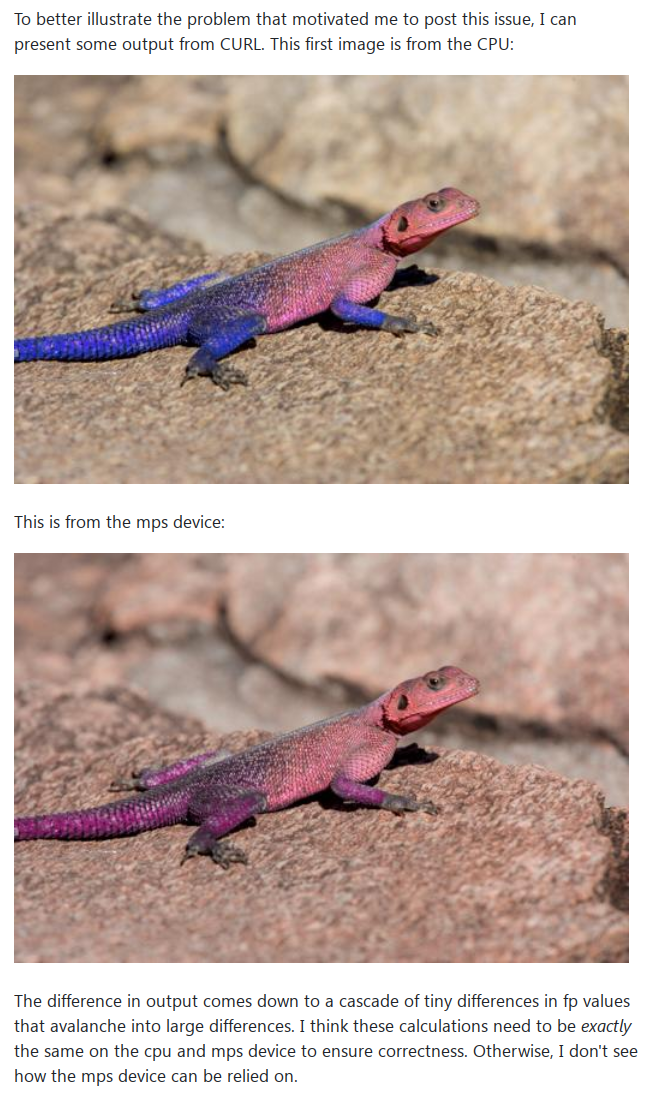
\includegraphics{images/math-fp-discrepancy-outcome-lizard.png}

This snapshot and the commentary come from this
\href{https://github.com/pytorch/pytorch/issues/84936\#issuecomment-1246084645}{PyTorch
Issue thread}.

If you're curious where I pulled this code from - this is a simplified
reduction of this original code in
\href{https://github.com/huggingface/transformers/blob/3f69f415adcbdaedec154ba8eac220ef3276975d/src/transformers/models/llama/modeling_llama.py\#L130}{modeling\_llama.py}:

\begin{Shaded}
\begin{Highlighting}[]
\KeywordTok{class}\NormalTok{ LlamaRotaryEmbedding(nn.Module):}
    \KeywordTok{def} \FunctionTok{\_\_init\_\_}\NormalTok{(}\VariableTok{self}\NormalTok{, dim, max\_position\_embeddings}\OperatorTok{=}\DecValTok{2048}\NormalTok{, base}\OperatorTok{=}\DecValTok{10000}\NormalTok{, device}\OperatorTok{=}\VariableTok{None}\NormalTok{):}
        \BuiltInTok{super}\NormalTok{().}\FunctionTok{\_\_init\_\_}\NormalTok{()}

        \VariableTok{self}\NormalTok{.dim }\OperatorTok{=}\NormalTok{ dim}
        \VariableTok{self}\NormalTok{.max\_position\_embeddings }\OperatorTok{=}\NormalTok{ max\_position\_embeddings}
        \VariableTok{self}\NormalTok{.base }\OperatorTok{=}\NormalTok{ base}
\NormalTok{        inv\_freq }\OperatorTok{=} \FloatTok{1.0} \OperatorTok{/}\NormalTok{ (}\VariableTok{self}\NormalTok{.base }\OperatorTok{**}\NormalTok{ (torch.arange(}\DecValTok{0}\NormalTok{, }\VariableTok{self}\NormalTok{.dim, }\DecValTok{2}\NormalTok{).}\BuiltInTok{float}\NormalTok{().to(device) }\OperatorTok{/} \VariableTok{self}\NormalTok{.dim))}
        \VariableTok{self}\NormalTok{.register\_buffer(}\StringTok{"inv\_freq"}\NormalTok{, inv\_freq, persistent}\OperatorTok{=}\VariableTok{False}\NormalTok{)}
\end{Highlighting}
\end{Shaded}




\end{document}
